\chapter{Interazione radiazione-materia}
In questo capitolo ci occuperemo dell'interazione delle particelle con la materia, verrà diviso in tre sezioni : 
\begin{itemize}
        \item interazione di particelle cariche;
        \item interazione di fotoni; 
        \item interazione di neutroni.
\end{itemize}
\section{Interazione di particelle cariche con la materia}
Immaginiamo una particella con carica $\textit{z}e$ e massa m che attraversa un materiale di lunghezza $\dd{x}$ composto da atomi con numero di massa A e densità $\rho$
come in figura.
Ci chiadiamo quanto sia l'energia che perde la particella nell'attraversare il tratto $\dd{x}$ : 
\begin{align*}
    \frac{\dd{E}}{\dd{x}}
\end{align*}
\subsection{Perdita di energia per ionizzazione : la formula di Bohr}
Durante la derivazione della formula di Rutherford abbiamo assunto che se la particella ha un'interazione con il nucleo dell'atomo, la particella non perde 
energia siccome il nucleo ha una massa molto maggiore ma, così facendo, stiamo trascurando la possibilità di trasferire energia agli elettroni che è ciò che 
andremo a trattare in questa sezione.\\
\begin{figure}[!h]
    \centering
    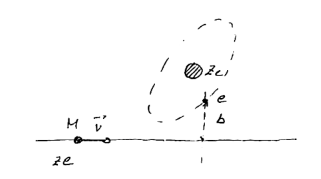
\includegraphics[scale=0.5]{ch6InterazioneMateria/BohrInterazione}
\end{figure}
\newpage
Dobbiamo calcolare l'energia cinetica ceduta all'elettrone ossia : 
\begin{align*}
        T_{e} = \frac{\Delta P_{e}^2}{2m_{e}}
\end{align*}
Per calcolare $\Delta P_{e}$ cambiamo sistema di riferimento in quello della particella dove quest'ultima è ferma e l'elettrone gli va incontro 
\begin{figure}[!h]
    \centering
    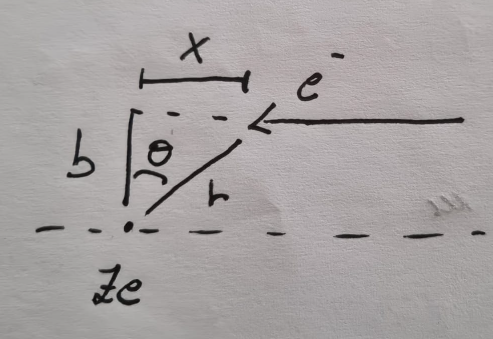
\includegraphics[scale=0.5]{ch6InterazioneMateria/CambioRiferimento}
\end{figure}

In una approssimazione non relativistica quindi possiamo vedere il tutto come un elettrone che passa nel campo culombiano di una particella con
carica $\textit{z}e$, attratto quindi da una forza : 
\begin{align*}
    F = \frac{\textit{z}e^2}{4\pi\epsilon_{0}}\frac{1}{r^2}
\end{align*}
possiamo dunque calcolare la quantità : 
\begin{align*}
        \Delta P_{e} &= \frac{\textit{z}e^2}{4\pi\epsilon_{0}}\int^{t}_{0}\frac{1}{r^2}\dd{t} \\
                     &= \frac{\textit{z}e^2}{4\pi\epsilon_{0}}\int^{\infty}_{-\infty}\frac{1}{r^2}\frac{\dd{x}}{v} \\
        \dd{t} &\rightarrow \frac{\dd{x}}{v} \tag*{Poichè v costante}
\end{align*}
Scomponiamo nelle due componenti considerando che $r = x^2 + b^2$ e che $(\Delta P)_{\parallel} = \Delta P\sin{\theta}$, $(\Delta P)_{\perp} = \Delta P\cos{\theta}$
otteniamo : 
\begin{align*}
        &(\Delta P)_{\parallel} =  \frac{\textit{z}e^2}{4\pi\epsilon_{0}v}\int\frac{1}{x^2 + b^2}\sin{\theta}\dd{x} = 0 \\
        &(\Delta P)_{\perp} =  \frac{\textit{z}e^2}{4\pi\epsilon_{0}v}\int\frac{1}{x^2 + b^2}\cos{\theta}\dd{x}
\end{align*}
\newpage
il secondo integrale lo calcoliamo sapendo che : 
\begin{align*}
        &\cos^2{\theta} = \frac{b^2}{x^2 + b^2} \\
        &\dd{x} = \frac{b}{\cos^2{\theta}}\dd{\theta}
\end{align*}
si ottiene : 
\begin{align*}
        (\Delta P)_{\perp} &=  \frac{\textit{z}e^2}{4\pi\epsilon_{0}vb}\int^{\frac{\pi}{2}}_{-\frac{\pi}{2}}\cos{\theta}\dd{\theta} \\
                           &= 2\frac{\textit{z}e^2}{4\pi\epsilon_{0}vb} \\
                           &= \frac{\textit{z}e^2}{4\pi\epsilon_{0}vb^2}\frac{2b}{v}
\end{align*}
\begin{tcolorbox}[colback=red!5!white,colframe=red!50!black,title=ATTENZIONE !]
nella formula sopra bisogna dire che : 
\begin{itemize}
        \item $ \frac{\textit{z}e^2}{4\pi\epsilon_{0}vb^2}$ = forza trasversale; 
        \item $\frac{2b}{v}$ = scattering time ; 
        \item abbiamo assunto che l'elettrone si muova su una linea dritta, ciò va bene se assumiamo che la velocità della particella sia molto maggiore 
                della velocità di orbita dell'elettrone.
\end{itemize}
\end{tcolorbox}

Troviamo così, nel caso non relativistico, l'energia persa : 
\begin{align*}
        \Delta T_{e} &= \frac{\Delta P_{e}^2}{2m_{e}} \\ 
                     &=\frac{2\textit{z}^2e^4}{m_{e}v^2b^2(4\pi\epsilon_{0})^2} 
\end{align*}
Introducendo $\beta = \frac{v}{c}$ e il raggio classico dell'elettrone $r_{e} = \frac{e^2}{4\pi\epsilon_{0}m_{e}c^2}$
\begin{align*}
        \Delta T_{e} &=  \frac{2\textit{z}^2e^4}{m_{e}c^2\beta^2b^2(4\pi\epsilon_{0})^2} \\
                     &= \frac{2\textit{z}^2m_{e}c^2}{\beta^2b^2}\qty[\frac{e^2}{4\pi\epsilon_{0}m_{e}c^2}]^2 \\
                     &= \frac{2\textit{z}^2m_{e}c^2}{\beta^2b^2}r_{e}^2
\end{align*}
\newpage
Dal punto di vista della particella incidente, il materiale che incontra può essere visto come un " fascio "
di elettroni distribuiti su una corona cilindrica a distanza comprese fra b e b + $\dd{b}$ come in figura
\begin{figure}[!h]
    \centering
    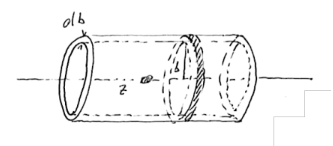
\includegraphics[scale=0.5]{ch6InterazioneMateria/DistribuzioneElettroni}
\end{figure}
Se $n_{e}$ è la densità degli elettroni nel materiale allora il numero di elettroni che 
la particella incontra in un tratto $\dd{x}$ è dato da : 
\begin{align*}
    \dd{N} = n_{e}V = n_{e}2\pi b\dd{b}\dd{x}
\end{align*}
Il valore dell'elemento di energia persa in un tratto infinitesimale $\dd{x}$ e dato il parametro di impatto 
\begin{align*}
    \frac{\dd[2]{E}}{\dd{x}\dd{b}} = n_{e}r_{e}^2m_{e}c^2\frac{4\pi}{b}\frac{z^2}{\beta^2}
\end{align*}
otteniamo quindi quello che volevamo cercare ossia l'energia persa per unità di lunghezza
\begin{align*}
        \frac{\dd{E}}{\dd{x}} &= n_{e}r_{e}^2m_{e}c^2\frac{4\pi z^2}{\beta^2}\int_{b_{min}}^{b_{max}}\frac{1}{b}\dd{b} \\[1em]
                              &= n_{e}r_{e}^2m_{e}c^2\frac{4\pi z^2}{\beta^2}\ln{\frac{b_{max}}{b_{min}}}
\end{align*}
Quello che bisogna fare ora è stimare $b_{min}$ e $b_{max}$.\\
\begin{itemize}
        \item Dato il principio di indeterminazione 
                \begin{align*}
                    \Delta p\Delta x = \hbar
                \end{align*}
            Se consideriamo $\Delta p$ come il momento dell'elettrone $p_{e}=m_{e}\gamma\beta c$
            otteniamo la risoluzione spaziale minima 
            \begin{align*}
                b_{min} = \frac{\hbar}{m_{e}\gamma\beta c}
            \end{align*}
    \item Come abbiamo detto, avendo considerato la traiettoria dell'elettrone sostanzialmente dritta 
        implica che lo scattering time definito sopra come $b/v$ deve essere relativamente piccolo rispetto al 
        tempo di rivoluzione dell'elettrone attorno all'atomo:
        \begin{align*}
            \gamma T_{e} = \gamma/w_{e}
        \end{align*}
        dove il fattore $\gamma$ tiene in considerazione della dilatazione del tempo.
        Come conseguenza si ottiene: 
        \begin{align*}
            b_{max} = \frac{\beta\gamma c}{w_{e}}
        \end{align*}
\end{itemize}
Otteniamo quindi la \textbf{formula di Bohr} : 
\begin{align*}
        \frac{\dd{E}}{\dd{x}} = 4\pi\rho N_{A}\frac{Z}{A}r_{e}^2m_{e}c^2\frac{z^2}{\beta^2}\ln{\frac{m_{e}c^2\beta^2\gamma^2}{\hbar w_{e}}}
\end{align*}
\subsection{Interpretazione della formula di Bohr}
La formula di Bohr dipende debolmente dal mezzo infatti, a parte costanti, la sua dipendenza 
è nel termine $Z/a$ che è nella stragrande maggioranza dei casi $\sim 1/2$. \\
Il termine più influente riguardante il mezzo è $\rho$, per tale motivo, per rendere la formula indipendente dal mezzo 
bersaglio di definisce : 
\begin{align*}
        \frac{1}{\rho}\frac{\dd{E}}{\dd{x}} &= 4\pi N_{A}\frac{Z}{A}r_{e}^2m_{e}c^2\frac{z^2}{\beta^2}\ln{\frac{m_{e}c^2\beta^2\gamma^2}{\hbar w_{e}}} \\[1em]
        \qty[\frac{1}{\rho}\frac{\dd{E}}{\dd{x}}] &= \frac{MeVcm^2}{g} 
\end{align*}
La dipendenza della particella è invece nel termine $Z^2/\beta^2$, ci sono due cose da dire: 
\begin{itemize}
        \item $Z^2$ : a parità di tutto, uno ione carbonio ( Z=6 ) scala 36 volte di più di un protone;
        \item la dipendenza da $\beta$ è scomoda poichè $0<\beta<1$ e per particelle relativistiche $\beta \sim 1$, conviene 
                esprimere dunque il grafico in funzione di $\beta\gamma$
\end{itemize}
\begin{figure*}[h!]
        \centering
        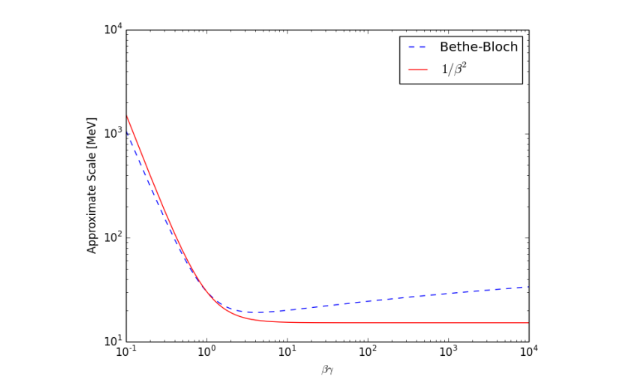
\includegraphics[scale=0.5]{ch6InterazioneMateria/BohrGrafico}
\end{figure*}

Per piccoli valori di energia, il termine dominante va come $1/\beta^2$ ad indicare che particelle lente perdono molta 
più energia rispetto a particelle più veloci.
A confronto con il semplice andamento di $1/\beta^2$ notiamo che vi è una piccola risalita nella perdita di energia, 
risalita dovuta al termine logaritmico, dovuto all'incremento del campo elettrico \\ " visto " dalla particella a velocità 
molto elevate, tale comportamento è denominato \textbf{risalita relativistica}.
\newpage
\subsection{La formula di Bethe-Bloch}
Una formula più generale, valida anche in casi realativistici, è quella di Bethe-Bloch:
\begin{align*}
    \frac{1}{\rho}\frac{\dd{E}}{\dd{x}} = C\frac{Z}{A}\frac{z^2}{\beta^2}\qty(\ln{\frac{2m_{e}c^2\beta^2\gamma^2}{I}}-\beta^2-\frac{\delta(\gamma)}{2})
\end{align*}
dove : 
\begin{itemize}
        \item abbiamo raccolto tutti le costanti $C=4\pi r_{e}^2c^2m_{e}N_{A} \simeq 0.307\frac{MeVcm^2}{g}$;
        \item la perdita di energia ha un minimo chiamato MIP \textit{ minimal-ionising particles } che 
                corrisponde a un $\beta\gamma \simeq 3$
\end{itemize}
\begin{figure}[!h]
    \centering
    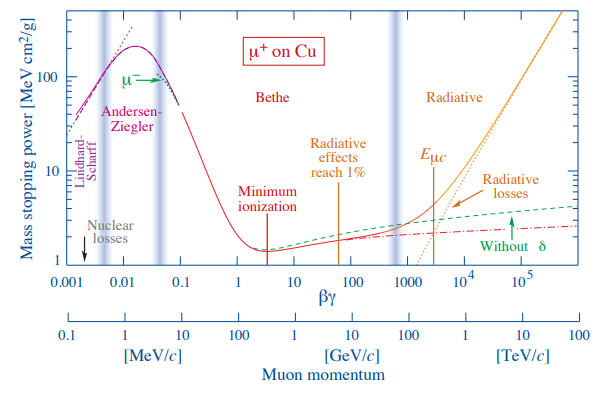
\includegraphics[scale=0.5]{ch6InterazioneMateria/BetheCompleta}
\end{figure}
Di questo grafico, che esprime la perdita di energia per ionizzazione su scale inferiori a quelle del momento del muone, 
la parte centrale fra le due bande grigie è ben descritta dalla formula di Bethe-Bloch.
\begin{itemize}
        \item Nella regione di sinistra, con valori di $\beta\gamma$ molto piccoli, il modello descritto fino ad ora non è 
                più valido, entrano in gioco effetti legati al fatto che la velocità del proiettile è paragonabile
                alla velocità di orbita degli elettroni;
        \item per grandi valori di $\beta\gamma$ il nostro modello non è valido, la perdita di energia è dovuta all'irraggiamento, 
                effetto di cui parleremo più avanti.
\end{itemize}
\begin{tcolorbox}[colback=red!5!white,colframe=red!50!black,title=ATTENZIONE !]
        La formula di Bethe-Bloch è un'espressione della perdita \textbf{media} di energia, siccome i processi di interazione
        fra particella e atomo è un processo stocastico, dobbiamo allora considerare anche la perdita di energia come casuale.
\end{tcolorbox}
\newpage
Per materiali spessi, il teorema del limite centrale ci assicura che le fluttuazioni siano gaussiane, questo non vale 
per materiali sottili, che seguiranno invece la distribuzione di Landau con code verso destra, ossia che vi sia un piccola 
probabilità di avere grandi perdite di energia.
\begin{figure}[!h]
    \centering
    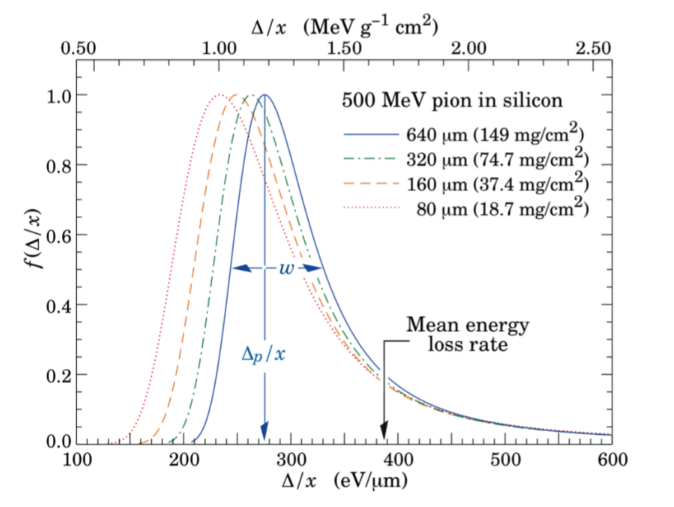
\includegraphics[scale=0.5]{ch6InterazioneMateria/Landau}
\end{figure}
\subsection{Il percorso residuo}
Si definisce come il percorso medio che compie una particella prima di perdere tutta la sue energia, quello che succede è che, 
perdendo energia, si risale la curva dell
\subsection{Effetto Cherenkov}
Quando una particella carica attraversa un mezzo polarizza gli atomi del materiale i quali rilasciano
radiazioni sotto forma di onde sferiche che hanno una velocità ( in un mezzo non dispersivo ) di :
\begin{align*}
        v_{g} = \frac{c}{n} \tag*{n è indice di rifrazione}
\end{align*}
\newpage
Quando la particella ha una velocità superiore a quella della luce nel mezzo vi è una convoluzione di queste onde sferiche che formano
un fronte d'onda, una luce quindi emessa ad un certo angolo $\theta_{c}$.
\begin{figure}[!h]
    \centering
    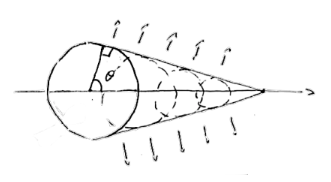
\includegraphics[scale=0.8]{ch6InterazioneMateria/Cherenkov}
\end{figure}

L'angolo di emissione è dato dalla relazione: 
\begin{align*}
        c\beta\cos{\theta_{c}} &= \frac{c}{n} \\[1em]
    \cos{\theta_{c}} &= \frac{1}{\beta n}
\end{align*}
L'equivalente meccanico di questo fenomeno è il boom supersonico.
